% ==============================================================================
% BAB III: METODOLOGI PENELITIAN
% Proposal Skripsi: Evaluasi Generalisasi Lintas Domain Model Analisis Sentimen Bahasa Madura
% Penulis: Muhammad Syawqi Muhtadabillah (NIM: 2302310276)
% ==============================================================================

\chapter{METODOLOGI PENELITIAN}

\section{Alur Penelitian}

Penelitian ini dirancang secara sistematis dengan menggunakan metode eksperimen komputasi untuk mengevaluasi generalisasi lintas domain model analisis sentimen bahasa Madura serta menguji efisiensi adaptasi bertahap pada model prapelatihan XLM-RoBERTa. Penulis menyajikan diagram alir pelaksanaan penelitian secara komprehensif pada \figurename~\ref{fig:alur_penelitian}.

\begin{figure}[H]
\centering
\begin{tikzpicture}[
    node distance=0.38cm and 1.0cm,
    font=\fontsize{8.5pt}{10.5pt}\selectfont,
    terminal/.style={rectangle, rounded corners=8pt, draw=black, thick, fill=gray!12, minimum width=5.0cm, minimum height=0.6cm, align=center},
    process/.style={rectangle, draw=black, thick, fill=white, minimum width=7.2cm, minimum height=0.65cm, align=center, inner sep=3.5pt},
    decision/.style={diamond, draw=black, thick, fill=gray!15, aspect=2.3, inner sep=2pt, align=center},
    line/.style={draw=black, -{Latex[length=2.2mm]}, thick}
]

% Node Tahapan
\node [terminal] (start) {\textbf{Mulai}};
\node [process, below=of start] (lit) {\textbf{Tahap 1: Studi Pustaka \& Identifikasi Kesenjangan Riset}\\(Kajian Model Lintas Domain \& Bahasa Madura Medsos)};
\node [process, below=of lit] (data) {\textbf{Tahap 2: Pengumpulan \& Kurasi Korpus Data}\\(NusaX Bahasa Madura \& Pengambilan Komentar TikTok)};
\node [process, below=of data] (prep) {\textbf{Tahap 3: Pra-pemrosesan Teks \& Anotasi Sentimen}\\(Pembersihan \textit{Noise} \& Pelabelan 3 Kelas Penutur Asli)};
\node [decision, below=0.38cm of prep] (kappa) {Uji Reliabilitas\\$\kappa \ge 0{,}65$?};
\node [process, left=0.9cm of kappa, text width=2.4cm] (rekon) {\textbf{Rekonsiliasi}\\Anotator Asli};
\node [process, below=0.38cm of kappa] (split) {\textbf{Tahap 4: Partisi Korpus Data Target}\\(Held-Out Test 200, Val Set 100, Pool Adaptasi 200)};
\node [process, below=of split] (train) {\textbf{Tahap 5: Pelatihan Baseline (S0) \& Zero-Shot (S1)}\\(Pelatihan di NusaX \& Evaluasi Langsung di TikTok)};
\node [process, below=of train] (adapt) {\textbf{Tahap 6: Adaptasi Domain Bertahap (S2a--S2d)}\\(Fine-Tuning Bertingkat: 10\%, 25\%, 50\%, 100\%)};
\node [process, below=of adapt] (eval) {\textbf{Tahap 7: Evaluasi Kinerja Kuantitatif \& Matriks Konfusi}\\(Akurasi, Presisi, Recall, Macro F1, Penurunan $\Delta_{\text{drop}}$)};
\node [process, below=of eval] (error) {\textbf{Tahap 8: Analisis Kesalahan Linguistik Kualitatif}\\(Taksonomi 4 Dimensi Kebahasaan \& Batas Representasi AI)};
\node [terminal, below=of error] (stop) {\textbf{Selesai}};

% Alur Panah
\path [line] (start) -- (lit);
\path [line] (lit) -- (data);
\path [line] (data) -- (prep);
\path [line] (prep) -- (kappa);
\path [line] (kappa) -- node[right, font=\scriptsize] {Ya} (split);
\path [line] (kappa) -- node[above, font=\scriptsize] {Tidak} (rekon);
\path [line] (rekon) |- (prep);
\path [line] (split) -- (train);
\path [line] (train) -- (adapt);
\path [line] (adapt) -- (eval);
\path [line] (eval) -- (error);
\path [line] (error) -- (stop);

\end{tikzpicture}
\caption{Diagram Alir Metodologi Penelitian}
\label{fig:alur_penelitian}
\end{figure}

Berdasarkan diagram alir metodologi penelitian pada \figurename~\ref{fig:alur_penelitian}, alur pelaksanaan riset dirancang secara sekuensial dan terstruktur ke dalam delapan tahapan utama. Tahapan tersebut mencakup pengumpulan data, kurasi korpus, pengujian reliabilitas kesepakatan anotator melalui koefisien Kappa, partisi korpus domain target yang terlindungi dari kebocoran data, pelatihan baseline in-domain, adaptasi bertahap few-shot, evaluasi kuantitatif, hingga taksonomi kesalahan linguistik. Rincian pelaksanaan dari masing-masing tahapan diuraikan sebagai berikut:
\begin{enumerate}
    \item \textbf{Tahap 1 (Studi Pustaka dan Identifikasi Masalah)}: Mengkaji landasan teoretis terkait pemrosesan bahasa alami (\textit{Natural Language Processing}), arsitektur model representasi prapelatihan multibahasa XLM-RoBERTa, dinamika pergeseran domain (\textit{domain shift}), serta karakteristik linguistik bahasa Madura informal pada media sosial.
    \item \textbf{Tahap 2 (Pengumpulan dan Kurasi Korpus Data)}: Mengunduh korpus acuan publik NusaX subset bahasa Madura yang mewakili domain formal sumber, serta mengumpulkan data komentar publik berbahasa Madura secara empiris dari platform TikTok yang mewakili domain target.
    \item \textbf{Tahap 3 (Pra-pemrosesan Teks dan Anotasi Ground Truth)}: Melakukan pembersihan data mentah (\textit{data cleaning}) meliputi penghapusan tautan URL, emoji, tanda pagar (\textit{hashtag}), dan nama pengguna (\textit{username}), kemudian melakukan pelabelan tiga kelas sentimen (positif, netral, negatif) bersama dua hingga tiga penutur asli bahasa Madura. Tingkat kesepakatan antar-anotator diuji menggunakan koefisien kesepakatan Kappa ($\kappa$). Apabila nilai $\kappa < 0{,}65$, dilakukan sesi rekonsiliasi hingga tercapai ambang reliabilitas minimum $\kappa \ge 0{,}65$.
    \item \textbf{Tahap 4 (Partisi Korpus Data Target)}: Membagi 500 sampel komentar TikTok berlabel secara terstrata (\textit{stratified split}) menjadi tiga himpunan terpisah: \textit{held-out test set} sebanyak 200 sampel (40\%) yang dikunci untuk pengujian akhir, \textit{target validation set} sebanyak 100 sampel (20\%) untuk pemantauan \textit{early stopping}, dan pool data latih sebanyak 200 sampel (40\%) untuk adaptasi bertingkat.
    \item \textbf{Tahap 5 (Pelatihan In-Domain Baseline dan Pengujian Zero-Shot)}: Melatih model fondasi XLM-RoBERTa pada data latih NusaX dengan validasi NusaX Val untuk menghasilkan model \textit{baseline} (S0), mengevaluasi performa puncaknya pada NusaX Test, kemudian menguji model tersebut secara langsung tanpa pelatihan tambahan pada data uji TikTok (S1) guna mengukur kesenjangan performa (\textit{cross-domain degradation}).
    \item \textbf{Tahap 6 (Adaptasi Domain Bertahap)}: Melakukan penyesuaian bobot (\textit{fine-tuning}) secara bertingkat menggunakan sub-kuota data adaptasi sebesar 10\% (S2a), 25\% (S2b), 50\% (S2c), dan 100\% (S2d) yang dievaluasi dengan bantuan \textit{early stopping} berbasis \textit{validation loss} target untuk mencegah \textit{overfitting}.
    \item \textbf{Tahap 7 (Evaluasi Kinerja Kuantitatif)}: Menghitung metrik performa komputasional mencakup \textit{Accuracy}, \textit{Precision}, \textit{Recall}, \textit{Macro F1-Score}, penurunan performa absolut ($\Delta_{\text{drop}}$), serta persentase penurunan ($\%\Delta_{\text{drop}}$) pada seluruh skenario eksperimen, yang dilengkapi penyajian matriks konfusi (\textit{confusion matrix}).
    \item \textbf{Tahap 8 (Analisis Kesalahan Linguistik Kualitatif)}: Mengekstrak seluruh sampel komentar yang salah diprediksi oleh model (\textit{false positives} dan \textit{false negatives}), kemudian mengklasifikasikan kesalahan tersebut ke dalam empat dimensi taksonomi kebahasaan Madura untuk mengidentifikasi keterbatasan mendasar dari representasi subkata model AI.
\end{enumerate}

\section{Lingkungan dan Instrumen Eksperimen}

Pelaksanaan eksperimen komputasi dalam penelitian ini memanfaatkan infrastruktur awan (\textit{cloud computing}) yang terintegrasi dengan akselerator grafis (\textit{GPU accelerator}) berkinerja tinggi serta ekosistem perangkat lunak sumber terbuka (\textit{open-source}) berbasis Python. Penulis merangkum spesifikasi perangkat keras dan perangkat lunak yang dialokasikan dalam penelitian pada \tablename~\ref{tab:lingkungan_komputasi}.

\begin{table}[H]
    \centering
    \small
    \renewcommand{\arraystretch}{1.08}
    \begin{tabularx}{\textwidth}{|>{\raggedright\arraybackslash}p{4.2cm}|>{\raggedright\arraybackslash}X|}
        \hline
        \rowcolor[gray]{0.85}
        \textbf{Komponen Sistem} & \textbf{Spesifikasi / Alokasi Komputasi} \\
        \hline
        Platform Komputasi & Google Colab Pro Compute Platform \\
        \hline
        Akselerator Grafis (GPU) & NVIDIA Tesla T4 / V100 / A100 (16 GB / 40 GB VRAM) \\
        \hline
        Memori Sistem (RAM) & High-Memory Instance (25 GB hingga 52 GB RAM) \\
        \hline
        Sistem Operasi Host & Linux Ubuntu 22.04 LTS (x86\_64) \\
        \hline
        Bahasa Pemrograman & Python 3.10+ \\
        \hline
        Kerangka Kerja Utama & PyTorch 2.2+ dan CUDA 12.1 \\
        \hline
        Pustaka NLP & Hugging Face \textit{transformers}, \textit{datasets}, \textit{evaluate}, \textit{accelerate} \\
        \hline
        Pustaka Evaluasi \& Visual & Scikit-Learn, Pandas, NumPy, Matplotlib, Seaborn \\
        \hline
        Model Fondasi & XLM-RoBERTa Base (\texttt{xlm-roberta-base}) \\
        \hline
        Arsitektur Enkoder & 12 Lapisan Transformer, 768 \textit{hidden dimension}, 12 \textit{attention heads}, $\approx 278 \times 10^6$ parameter \\
        \hline
    \end{tabularx}
    \caption{Spesifikasi Lingkungan dan Instrumen Komputasi Eksperimen}
    \label{tab:lingkungan_komputasi}
\end{table}

Berdasarkan \tablename~\ref{tab:lingkungan_komputasi}, pemanfaatan akselerator GPU berkapasitas VRAM besar sangat krusial guna menampung struktur parameter model XLM-RoBERTa yang mencapai sekitar 278 juta parameter serta menjaga kestabilan alokasi memori selama proses perambatan maju (\textit{forward pass}) dan perambatan mundur (\textit{backward pass}) dengan ukuran \textit{batch} yang telah ditentukan.

\section{Akuisisi Data dan Partisi Korpus}

Penelitian ini menggunakan dua korpus teks dengan karakteristik kebahasaan yang kontras, yaitu domain sumber (\textit{source domain}) yang bersifat baku dan terstruktur serta domain target (\textit{target domain}) yang bersifat informal dan dinamis.

\subsection{Domain Sumber: Korpus NusaX Bahasa Madura}

Korpus domain sumber diperoleh dari dataset acuan publik NusaX subset bahasa Madura \citep{winata2023nusax}. Korpus ini tersusun atas kalimat ulasan yang diterjemahkan secara manual ke dalam bahasa Madura dengan mengikuti kaidah ejaan ortografi standar. Korpus NusaX bahasa Madura menyediakan 1.000 sampel teks dengan distribusi tiga kelas sentimen yang seimbang (\textit{balanced dataset}):
\begin{itemize}
    \item Sentimen Positif: $\approx 33{,}3\%$ (333 sampel)
    \item Sentimen Netral: $\approx 33{,}4\%$ (334 sampel)
    \item Sentimen Negatif: $\approx 33{,}3\%$ (333 sampel)
\end{itemize}

Sesuai partisi kanonikal yang ditetapkan dalam penelitian NusaX \citep{winata2023nusax}, dataset ini terbagi menjadi 500 sampel data latih (\textit{train set}), 100 sampel data validasi (\textit{development set}), dan 400 sampel data uji (\textit{test set}).

\subsection{Domain Target: Korpus Komentar TikTok Berbahasa Madura}

Korpus domain target dihimpun secara empiris dari platform media sosial TikTok \citep{luther2026analisis, saputra2026reaksi}. Pengumpulan data dilakukan melalui penelusuran manual terhadap video publik bertopik interaksi lokal masyarakat Madura yang memuat interaksi berbasis bahasa Madura pada kolom komentar. Cakupan konten video dibuka secara luas (meliputi konten sketsa komedi, kuliner, pariwisata, kegiatan kemasyarakatan, dan wacana publik) guna menjaring variasi leksikal yang merefleksikan kondisi nyata bahasa Madura di ruang siber.

Korpus target yang berhasil dihimpun dan dikurasi berjumlah 500 komentar unik. Prosedur penyaringan data awal (\textit{data filtering}) dilakukan melalui tahapan berikut:
\begin{itemize}
    \item Menghilangkan komentar duplikat (\textit{deduplication}).
    \item Menghapus entri yang murni berupa tautan promosi, spam bot, atau deretan emotikon tanpa teks bermakna.
    \item Melakukan verifikasi leksikal bersama penutur asli untuk memastikan kehadiran unsur kosakata bahasa Madura (seperti partikel penegas, kata ganti, maupun kata penunjuk lokal) dalam komentar yang menggunakan gaya campur kode (\textit{code-mixing}).
\end{itemize}

\subsection{Skema Partisi Korpus Domain Target dan Peran Validation Set}

Untuk menjamin keabsahan metodologis dan mencegah kebocoran informasi (\textit{data leakage}), 500 sampel komentar TikTok berlabel dibagi ke dalam tiga subset independen menggunakan metode pemisahan terstrata (\textit{stratified split}):
\begin{enumerate}
    \item \textbf{Held-Out Test Set (40\% / 200 sampel)}: Sebanyak 200 komentar dialokasikan khusus sebagai himpunan uji akhir domain target. Subset ini dikunci secara ketat dan tidak pernah dilibatkan dalam proses pelatihan maupun pemilihan \textit{checkpoint} model, sehingga evaluasi lintas skenario bersifat objektif.
    \item \textbf{Target Validation Set (20\% / 100 sampel)}: Sebanyak 100 komentar dialokasikan sebagai data validasi domain target. Keberadaan subset ini memegang peran krusial:
    \begin{itemize}
        \item Menyediakan sinyal objektif untuk memantau nilai \textit{validation loss} dan mengendalikan mekanisme penghentian awal (\textit{early stopping}) selama proses penyesuaian bobot model.
        \item Mencegah kebocoran data uji karena penentuan model terbaik tidak mengacu pada \textit{held-out test set}.
        \item Mengeliminasi bias evaluasi domain sumber yang dapat terjadi apabila adaptasi hanya divalidasi menggunakan NusaX Val yang memiliki ragam bahasa berbeda.
    \end{itemize}
    \item \textbf{Pool Data Latih Adaptasi (40\% / 200 sampel)}: Sebanyak 200 komentar dialokasikan sebagai bank data latih domain target yang dipartisi secara bersarang (\textit{nested stratified subsets}) ke dalam empat kuota latihan:
    \begin{itemize}
        \item Sub-kuota 10\% ($S_{10\%}$): 20 sampel komentar untuk menguji efektivitas adaptasi data sangat minim (\textit{few-shot learning}).
        \item Sub-kuota 25\% ($S_{25\%}$): 50 sampel komentar untuk mengamati respons awal kurva adaptasi pada kuartal pertama data latih.
        \item Sub-kuota 50\% ($S_{50\%}$): 100 sampel komentar untuk mengevaluasi pemulihan performa pada separuh kuota data target.
        \item Sub-kuota 100\% ($S_{100\%}$): 200 sampel komentar untuk menetapkan batas atas kinerja adaptasi terawasi penuh pada domain target.
    \end{itemize}
\end{enumerate}

Penulis menyajikan rekapitulasi struktur alokasi dan pembagian himpunan data penelitian pada \tablename~\ref{tab:partisi_data}.

\begin{table}[H]
    \centering
    \footnotesize
    \setlength{\tabcolsep}{4pt}
    \renewcommand{\arraystretch}{1.08}
    \begin{tabularx}{\textwidth}{|>{\raggedright\arraybackslash}p{3.2cm}|>{\centering\arraybackslash}p{2.6cm}|>{\centering\arraybackslash}p{2.2cm}|>{\raggedright\arraybackslash}X|}
        \hline
        \rowcolor[gray]{0.85}
        \textbf{Kategori Domain} & \textbf{Himpunan Data} & \textbf{Volume} & \textbf{Fungsi Pengujian} \\
        \hline
        Domain Sumber (NusaX) & NusaX Train & 500 sampel & Pelatihan model \textit{baseline} awal (S0) \\
        \hline
        Domain Sumber (NusaX) & NusaX Val & 100 sampel & Validasi \& \textit{early stopping} model \textit{baseline} \\
        \hline
        Domain Sumber (NusaX) & NusaX Test & 400 sampel & Pengujian \textit{in-domain baseline} (S0) \\
        \hline
        Domain Target (TikTok) & Held-Out Test Set & 200 sampel (40\%) & Pengujian objektif lintas domain (S1 \& S2a--S2d) \\
        \hline
        Domain Target (TikTok) & Target Val Set & 100 sampel (20\%) & Validasi \& \textit{early stopping} adaptasi target \\
        \hline
        Domain Target (TikTok) & Pool Adaptasi 10\% & 20 sampel & Evaluasi adaptasi \textit{few-shot} target (S2a) \\
        \hline
        Domain Target (TikTok) & Pool Adaptasi 25\% & 50 sampel & Evaluasi adaptasi kuartal target (S2b) \\
        \hline
        Domain Target (TikTok) & Pool Adaptasi 50\% & 100 sampel & Evaluasi adaptasi paruh data target (S2c) \\
        \hline
        Domain Target (TikTok) & Pool Adaptasi 100\% & 200 sampel & Evaluasi adaptasi penuh target (S2d) \\
        \hline
    \end{tabularx}
    \caption{Rencana Partisi Data Penelitian}
    \label{tab:partisi_data}
\end{table}

Berdasarkan \tablename~\ref{tab:partisi_data}, partisi data disusun secara berimbang agar seluruh proses pelatihan, validasi, dan pengujian dapat berjalan secara sistematis tanpa ada tumpang tindih data antartahapan pengujian.

\section{Prosedur Anotasi dan Uji Reliabilitas Label}

Guna menjamin mutu korpus data target, proses pelabelan dilakukan secara independen oleh dua hingga tiga penutur asli bahasa Madura yang memiliki kompetensi kebahasaan serta latar belakang pendidikan tinggi. Keterlibatan penutur asli sangat penting untuk memahami konteks kultural dialek Madura Timur (Sumenep dan Pamekasan) maupun Madura Barat (Bangkalan dan Sampang) \citep{cahyawijaya2023nusawrites, winata2023nusax}.

\subsection{Pedoman Anotasi Sentimen (Annotation Guidelines)}

Anotasi sentimen dilaksanakan dengan mempedomani ketentuan baku tiga kelas sentimen berikut:
\begin{enumerate}
    \item \textbf{Sentimen Positif}: Komentar yang mengekspresikan apresiasi, pujian, kekaguman, doa, rasa syukur, kebahagiaan, dukungan afektif, atau kepuasan. Contoh: ``\textit{Bagus ontong konten reya, bender mon oreng Madure juko'na sanget rajin}'' (Bagus sekali konten ini, benar jika orang Madura kerjanya sangat rajin).
    \item \textbf{Sentimen Netral}: Komentar yang bersifat informatif murni, pertanyaan faktual mengenai lokasi atau harga, pernyataan umum tanpa muatan emosi, atau klarifikasi logistik. Contoh: ``\textit{Dimma kennengenna reya kak? Lokasina e Songennep apa e Mekkasen?}'' (Di mana tempatnya ini kak? Lokasinya di Sumenep apa di Pamekasan?).
    \item \textbf{Sentimen Negatif}: Komentar yang mengekspresikan kekecewaan, ketidaksetujuan, kemarahan, cemoohan, kritik pedas, atau penghinaan. Contoh: ``\textit{Jelek sanget kelakuanna, ta' tao todus ka oreng towa}'' (Jelek sekali perbuatannya, tidak punya rasa malu kepada orang tua).
\end{enumerate}

Khusus untuk kalimat yang mengandung majas sarkasme atau satir kultural, label ditentukan berdasarkan intensi pragmatik penutur yang tersirat di balik konteks kalimat, bukan semata-mata arti leksikal harfiah.

\subsection{Pengukuran Kesepakatan Antar-Anotator}

Tingkat reliabilitas anotasi diukur secara matematis menggunakan koefisien kesepakatan Cohen's Kappa atau Fleiss' Kappa sesuai Persamaan~\eqref{eq:cohen_kappa}. Nilai ambang batas reliabilitas ditetapkan pada $\kappa \ge 0{,}65$ (\textit{substantial agreement}). Apabila terdapat selisih pelabelan antar-anotator, penulis menyelenggarakan sesi rekonsiliasi bersama para anotator untuk mengkaji konteks kebahasaan dan menyepakati label kebenaran akhir (\textit{ground truth consensus}).

\section{Prosedur Pelatihan dan Protokol Adaptasi Domain}

Arsitektur model komputasi yang diterapkan berpusat pada model fondasi XLM-RoBERTa Base yang dipadukan dengan lapisan klasifikasi linier (\textit{Linear Classification Head}) di atas representasi vektor token klasifikasi $\mathbf{h}_{\langle s \rangle}$ (ekuivalen dengan token $\mathbf{h}_{\text{[CLS]}}$ pada BERT). Pemetaan keluaran klasifikasi ke dalam probabilitas tiga kelas dilakukan melalui fungsi aktivasi Softmax. Penulis menyajikan diagram alir rancangan metode pemodelan klasifikasi menggunakan arsitektur XLM-RoBERTa pada \figurename~\ref{fig:flowchart_metode}.

\begin{figure}[H]
\centering
\begin{tikzpicture}[
    node distance=0.38cm,
    font=\fontsize{8.5pt}{10.5pt}\selectfont,
    io/.style={trapezium, trapezium left angle=75, trapezium right angle=105, draw=black, thick, fill=gray!12, minimum height=0.6cm, align=center, inner sep=3.5pt},
    proc/.style={rectangle, draw=black, thick, fill=white, minimum width=7.2cm, minimum height=0.6cm, align=center, inner sep=3.5pt},
    line/.style={draw=black, -{Latex[length=2.2mm]}, thick}
]

\node [io] (in) {\textbf{Input}: Kalimat Komentar Teks Berbahasa Madura ($\mathbf{x}$)};
\node [proc, below=of in] (clean) {Pembersihan \& Normalisasi Teks (\textit{Data Cleaning})};
\node [proc, below=of clean] (bpe) {Tokenisasi BPE SentencePiece (Kosakata 250.000 Subkata)};
\node [proc, below=of bpe] (emb) {Lapisan Input: \textit{Token Embedding} + \textit{Positional Encoding}};
\node [proc, below=of emb] (enc) {12 Lapisan Transformer Enkoder ($d_{\text{model}}=768$, 12 \textit{Attention Heads})};
\node [proc, below=of enc] (cls) {Ekstraksi Representasi Vektor Klasifikasi $\mathbf{h}_{\langle s \rangle} \in \mathbb{R}^{768}$};
\node [proc, below=of cls] (drop) {Lapisan \textit{Dropout} ($p=0{,}1$) untuk Regularisasi};
\node [proc, below=of drop] (linear) {Lapisan Linear Klasifikasi ($\mathbf{W} \in \mathbb{R}^{3 \times 768} + \mathbf{b}$)};
\node [proc, below=of linear] (softmax) {Aktivasi Softmax: $P(y=c|\mathbf{x}) = \frac{\exp(z_c)}{\sum_{j=1}^3 \exp(z_j)}$};
\node [io, below=of softmax] (out) {\textbf{Output}: Distribusi Probabilitas \& Prediksi Kelas $\hat{y}$};
\node [proc, below=of out] (loss) {Perhitungan \textit{Cross-Entropy Loss} \& Optimasi Bobot AdamW};

\path [line] (in) -- (clean);
\path [line] (clean) -- (bpe);
\path [line] (bpe) -- (emb);
\path [line] (emb) -- (enc);
\path [line] (enc) -- (cls);
\path [line] (cls) -- (drop);
\path [line] (drop) -- (linear);
\path [line] (linear) -- (softmax);
\path [line] (softmax) -- (out);
\path [line] (out) -- (loss);

\end{tikzpicture}
\caption{Diagram Alir Metode Klasifikasi dan Pelatihan Model XLM-RoBERTa}
\label{fig:flowchart_metode}
\end{figure}

Berdasarkan diagram alir metode pada \figurename~\ref{fig:flowchart_metode}, alur pemodelan memperlihatkan transformasi komputasi yang runtut dari tahap masukan teks mentah hingga penetapan keputusan sentimen akhir. Kalimat komentar masukan bahasa Madura terlebih dahulu melalui pembersihan derau ortografi sebelum dipecah menjadi rangkaian token subkata oleh \textit{tokenizer} BPE SentencePiece dengan modal 250.000 kosakata bersama. Rangkaian token tersebut ditransformasikan ke dalam representasi vektor padat melalui lapisan \textit{embedding}, kemudian diproses oleh 12 lapisan enkoder \textit{transformer} menggunakan mekanisme atensi mandiri multi-kepala. Vektor representasi status tersembunyi token klasifikasi awal $\mathbf{h}_{\langle s \rangle}$ diekstraksi dan dilewatkan pada lapisan \textit{dropout} serta \textit{linear classifier} untuk menghasilkan nilai \textit{logits} sebelum diubah menjadi probabilitas tiga kelas sentimen melalui fungsi aktivasi Softmax.

\subsection{Konfigurasi Hiperparameter}

Konfigurasi parameter turunan dalam pelatihan ini ditetapkan berdasarkan kaidah baku penyesuaian halus (\textit{fine-tuning}) arsitektur Transformer yang merujuk pada literatur empiris terkini \citep{darnoto2026language, luther2026analisis}. Penulis menyajikan rincian konfigurasi hiperparameter pelatihan pada \tablename~\ref{tab:hiperparameter}.

\begin{table}[H]
    \centering
    \footnotesize
    \setlength{\tabcolsep}{4pt}
    \renewcommand{\arraystretch}{1.08}
    \begin{tabularx}{\textwidth}{|>{\raggedright\arraybackslash}p{5.5cm}|>{\raggedright\arraybackslash}X|}
        \hline
        \rowcolor[gray]{0.85}
        \textbf{Hiperparameter} & \textbf{Nilai Konfigurasi} \\
        \hline
        Model Fondasi & \texttt{xlm-roberta-base} \\
        \hline
        Ukuran Kosakata Tokenizer & 250.000 subkata (\textit{Byte-Pair Encoding}) \\
        \hline
        Panjang Sekuens Maksimum (\textit{Max Length}) & 128 token \\
        \hline
        Ukuran Batch Pelatihan (\textit{Batch Size}) & 16 / 32 sampel per iterasi \\
        \hline
        Optimasi Algoritma & AdamW (\textit{Adam with Decoupled Weight Decay}) \\
        \hline
        Laju Pembelajaran (\textit{Learning Rate}) & $2 \times 10^{-5}$ (\texttt{2e-5}) \\
        \hline
        Jadwal Laju Pembelajaran (\textit{LR Scheduler}) & Linear Decay with Warmup (proporsi pemanasan 10\%) \\
        \hline
        Pembusukan Bobot (\textit{Weight Decay}) & 0,01 \\
        \hline
        Jumlah Epoch Maksimum & 3 hingga 5 epoch \\
        \hline
        Kriteria Penghentian Awal (\textit{Early Stopping}) & Berbasis Validation Loss (toleransi \textit{patience} = 2 epoch) \\
        \hline
        Fungsi Kerugian (\textit{Loss Function}) & \textit{Cross-Entropy Loss} \\
        \hline
    \end{tabularx}
    \caption{Konfigurasi Hiperparameter Pelatihan Model XLM-RoBERTa}
    \label{tab:hiperparameter}
\end{table}

Berdasarkan \tablename~\ref{tab:hiperparameter}, penggunaan laju pembelajaran kecil sebesar $2 \times 10^{-5}$ dipadukan dengan algoritma AdamW bertujuan untuk mencegah terjadinya fenomena kelupaan katastropik (\textit{catastrophic forgetting}) pada representasi pengetahuan multibahasa yang telah dipelajari model sebelumnya.

\subsection{Matriks Protokol Pengujian Eksperimental}

Guna menjawab seluruh rumusan masalah penelitian secara tuntas, penulis merancang enam skenario eksperimen komparatif. Penulis menyajikan matriks skenario eksperimen penelitian secara rinci pada \tablename~\ref{tab:skenario_eksperimen}.

\begin{table}[H]
    \centering
    \footnotesize
    \setlength{\tabcolsep}{3.5pt}
    \renewcommand{\arraystretch}{1.08}
    \begin{tabularx}{\textwidth}{|c|>{\raggedright\arraybackslash}p{2.8cm}|>{\raggedright\arraybackslash}p{2.8cm}|>{\raggedright\arraybackslash}p{2.1cm}|>{\raggedright\arraybackslash}X|}
        \hline
        \rowcolor[gray]{0.85}
        \textbf{Kode} & \textbf{Nama Skenario} & \textbf{Korpus Latih \& Val} & \textbf{Korpus Uji} & \textbf{Tujuan \& Hipotesis Pengujian} \\
        \hline
        S0 & In-Domain Baseline & Latih: NusaX (500)\newline Val: NusaX (100) & NusaX Test (400) & Mengukur batas kinerja puncak model pada domain formal sumber. \\
        \hline
        S1 & Zero-Shot Cross-Domain & Latih: NusaX (500)\newline Val: NusaX (100) & TikTok Test (200) & Mengukur degradasi performa ($\Delta_{\text{drop}}$) akibat pergeseran domain. \\
        \hline
        S2a & Adaptasi 10\% Data & Latih: NusaX + 20 TikTok\newline Val: TikTok (100) & TikTok Test (200) & Menguji efektivitas adaptasi data sangat minimal (\textit{few-shot}). \\
        \hline
        S2b & Adaptasi 25\% Data & Latih: NusaX + 50 TikTok\newline Val: TikTok (100) & TikTok Test (200) & Mengamati kurva pemulihan F1 pada kuartal pertama data adaptasi. \\
        \hline
        S2c & Adaptasi 50\% Data & Latih: NusaX + 100 TikTok\newline Val: TikTok (100) & TikTok Test (200) & Mengevaluasi respons pemulihan performa pada separuh kuota data target. \\
        \hline
        S2d & Adaptasi 100\% Data & Latih: NusaX + 200 TikTok\newline Val: TikTok (100) & TikTok Test (200) & Mengukur batas performa optimal adaptasi penuh domain target. \\
        \hline
    \end{tabularx}
    \caption{Matriks Skenario Eksperimen Penelitian}
    \label{tab:skenario_eksperimen}
\end{table}

Berdasarkan \tablename~\ref{tab:skenario_eksperimen}, skenario S0 dan S1 berfungsi sebagai dasar komparasi untuk menghitung degradasi lintas domain, sedangkan skenario S2a hingga S2d memetakan dinamika kurva efisiensi sampel adaptasi bertahap.

Untuk menghubungkan seluruh proses evaluasi kinerja kuantitatif dengan analisis linguistik kualitatif, penulis menyusun model evaluasi komprehensif. Penulis menyajikan skema rancangan model evaluasi penelitian pada \figurename~\ref{fig:model_evaluasi}.

\begin{figure}[H]
\centering
\begin{tikzpicture}[
    font=\fontsize{8.5pt}{10.5pt}\selectfont,
    node distance=0.4cm and 0.9cm,
    header/.style={rectangle, draw=black, thick, fill=gray!20, minimum width=5.2cm, minimum height=0.65cm, align=center, font=\bfseries\footnotesize},
    block/.style={rectangle, draw=black, fill=white, minimum width=5.0cm, minimum height=0.6cm, align=center, inner sep=3pt},
    dim/.style={rectangle, draw=black, fill=gray!6, minimum width=4.8cm, minimum height=0.52cm, align=left, inner sep=3pt, font=\scriptsize},
    line/.style={draw=black, -{Latex[length=2.2mm]}, thick}
]

% Pilar Kuantitatif
\node [header] (h_kuan) {Pilar 1: Evaluasi Kuantitatif};
\node [block, below=0.35cm of h_kuan] (k_gap) {Pengukuran Kesenjangan Domain\\(S0 Baseline vs S1 Zero-Shot)};
\node [block, below=0.3cm of k_gap] (k_adapt) {Efisiensi Sampel Adaptasi Bertahap\\(S2a 10\%, S2b 25\%, S2c 50\%, S2d 100\%)};
\node [block, below=0.3cm of k_adapt] (k_metrik) {Metrik Komputasi \& Kurva:\\Akurasi, Presisi, Recall, Macro F1, $\Delta_{\text{drop}}$};

% Pilar Kualitatif
\node [header, right=1.6cm of h_kuan] (h_kual) {Pilar 2: Evaluasi Kualitatif};
\node [block, below=0.35cm of h_kual] (q_sample) {Ekstraksi Sampel Gagal Prediksi\\(\textit{False Positive} \& \textit{False Negative})};
\node [block, below=0.3cm of q_sample] (q_tax) {Taksonomi 4 Dimensi Kesalahan\\Linguistik Bahasa Madura};
\node [dim, below=0.25cm of q_tax] (d1) {1. Slang Medsos (\textit{onggu}, \textit{le}, \textit{jeh})};
\node [dim, below=0.15cm of d1] (d2) {2. Campur Kode (Madura-Indo-Jawa)};
\node [dim, below=0.15cm of d2] (d3) {3. Ejaan Non-Baku (\textit{bhungah} $\to$ bunga)};
\node [dim, below=0.15cm of d3] (d4) {4. Sarkasme \& Satir Kultural};

% Alur Panah Kuantitatif
\path [line] (h_kuan) -- (k_gap);
\path [line] (k_gap) -- (k_adapt);
\path [line] (k_adapt) -- (k_metrik);

% Alur Panah Kualitatif
\path [line] (h_kual) -- (q_sample);
\path [line] (q_sample) -- (q_tax);
\path [line] (q_tax) -- (d1);
\path [line] (d1) -- (d2);
\path [line] (d2) -- (d3);
\path [line] (d3) -- (d4);

% Hubungan Integrasi
\path [line, dashed] (k_adapt.east) -- node[above, font=\scriptsize, align=center] {Sampel\\Salah Prediksi} (q_sample.west);

\end{tikzpicture}
\caption{Skema Model Evaluasi Kinerja Kuantitatif dan Taksonomi Kesalahan Kualitatif}
\label{fig:model_evaluasi}
\end{figure}

Berdasarkan skema model evaluasi pada \figurename~\ref{fig:model_evaluasi}, kerangka penilaian kinerja dalam penelitian ini mengintegrasikan dua pilar utama yang saling melengkapi. Pilar 1 berfokus pada evaluasi kuantitatif komputasional yang mengukur besaran degradasi performa lintas domain ($\Delta_{\text{drop}}$) dan persentase penurunan ($\%\Delta_{\text{drop}}$) dari perbandingan skenario S0 dan S1, serta memetakan efisiensi sampel adaptasi bertahap pada skenario S2a hingga S2d melalui kurva metrik Macro F1. Pilar 2 berfokus pada evaluasi kualitatif linguistik melalui ekstraksi sampel salah prediksi (\textit{false positives} dan \textit{false negatives}), yang kemudian diklasifikasikan ke dalam taksonomi empat dimensi kebahasaan Madura guna mengidentifikasi batas representasi leksikal model prapelatihan.

\subsection{Metode Analisis Kesalahan Linguistik (Qualitative Error Taxonomy)}

Untuk melengkapi interpretasi statistik kuantitatif, analisis kesalahan kualitatif dirancang guna mengungkap keterbatasan pemahaman model terhadap struktur bahasa daerah non-baku. Prosedur taksonomi kesalahan linguistik dilaksanakan melalui tiga tahapan kerja:
\begin{enumerate}
    \item \textbf{Ekstraksi Sampel Gagal Prediksi}: Mengidentifikasi dan memilah seluruh baris komentar TikTok di mana label hasil prediksi model tidak sesuai dengan label kebenaran (\textit{ground truth}) pada pengujian S1 dan S2a hingga S2d.
    \item \textbf{Pengelompokan ke dalam Empat Dimensi Kesalahan}: Setiap data salah prediksi dipetakan ke dalam taksonomi kesalahan kebahasaan Madura:
    \begin{itemize}
        \item \textbf{Dimensi 1 (Kosakata Informal dan Slang Medsos)}: Kemunculan partikel penegas emosional dan kata sapaan khas (seperti \textit{onggu}, \textit{le}, \textit{jeh}, \textit{tretan}, \textit{cak}) yang memicu kekeliruan prediksi valensi sentimen \citep{arifin2026heuristic}.
        \item \textbf{Dimensi 2 (Campur Kode / Code-Mixing)}: Sisipan kosakata bahasa Indonesia dan bahasa Jawa yang bercampur secara acak dalam satu klausa bahasa Madura sehingga mengaburkan konteks kalimat bagi \textit{tokenizer} \citep{syauri2026analisis}.
        \item \textbf{Dimensi 3 (Variasi Ejaan Ortografi Tidak Baku)}: Penulisan kata yang menyimpang dari ejaan fonologis resmi, seperti penulisan kata \textit{bhungah} menjadi bunga, atau kata \textit{dhelem} menjadi delem, yang memicu fragmentasi subkata berlebihan \citep{arifin2026heuristic, firmansyah2021klasifikasi}.
        \item \textbf{Dimensi 4 (Sarkasme dan Satir Kultural)}: Kalimat yang memuat leksikon bernada positif (seperti ``\textit{hebat}'' atau ``\textit{penter onggu}'') namun ditujukan untuk mencemooh atau menyindir secara tersirat \citep{luther2026analisis, saputra2026reaksi}.
    \end{itemize}
    \item \textbf{Analisis Distribusi Frekuensi Kesalahan}: Menghitung persentase kemunculan masing-masing dimensi kesalahan sebelum dan sesudah adaptasi bertahap untuk menilai dimensi bahasa mana yang berhasil dipulihkan oleh data latih target dan dimensi mana yang tetap menjadi kendala permanen bagi model.
\end{enumerate}

\section{Perancangan Sistem dan Antarmuka MadSent}

\subsection{Integrasi Model XLM-RoBERTa dengan Backend Flask}

Implementasi sistem inferensi penelitian diwujudkan melalui pengembangan aplikasi web bernama MadSent (\textit{Madurese Sentiment Analysis}). Lingkungan komputasi Google Colab Pro digunakan sebagai platform pelatihan dan penyesuaian bobot (\textit{fine-tuning}), sedangkan kerangka kerja Flask digunakan sebagai \textit{backend} server lokal yang melayani permintaan inferensi sentimen teks secara mandiri.

Seluruh berkas \textit{checkpoint} model hasil pelatihan (mencakup bobot PyTorch, konfigurasi tokenisasi BPE SentencePiece, serta kamus pemetaan label) disimpan dan dimuat ke dalam memori kerja aplikasi Flask. Ketika pengguna memasukkan kalimat komentar berbahasa Madura melalui antarmuka pengguna, \textit{backend} Flask mengeksekusi pra-pemrosesan teks, melakukan tokenisasi, menjalankan perambatan maju (\textit{forward pass}) pada model terpilih, menghitung skor keyakinan (\textit{confidence score}) menggunakan fungsi Softmax, serta mencatat hasil prediksi ke dalam basis data riwayat inferensi.

\subsection{Pemodelan Berorientasi Objek Sistem MadSent}

Untuk menggambarkan fungsionalitas sistem secara terstruktur, perancangan perangkat lunak MadSent dimodelkan menggunakan diagram UML (\textit{Unified Modeling Language}) standar, yaitu diagram \textit{use case} dan diagram aktivitas (\textit{activity diagram}).

\subsubsection{Diagram Use Case Sistem MadSent}

Diagram \textit{use case} menyajikan batasan sistem serta interaksi fungsional antara pengguna (peneliti) dengan fungsionalitas sistem MadSent. Penulis menyajikan diagram \textit{use case} sistem MadSent pada \figurename~\ref{fig:usecase_madsent}.

\begin{figure}[H]
\centering
\begin{tikzpicture}[
    font=\fontsize{8.5pt}{10.5pt}\selectfont,
    actor/.style={circle, draw=black, thick, minimum size=0.75cm},
    usecase/.style={ellipse, draw=black, thick, fill=white, minimum width=4.0cm, minimum height=0.75cm, align=center, inner sep=2pt},
    system/.style={rectangle, draw=black, thick, fill=gray!4, minimum width=7.2cm, minimum height=8.2cm}
]

% Boundary Sistem
\node [system] (sys) at (3.6, -3.5) {};
\node [anchor=north west, font=\bfseries\footnotesize] at (sys.north west) {Sistem Analisis Sentimen MadSent};

% Actor Peneliti
\node [actor] (head) at (-1.6, -3.2) {};
\draw [thick] (head.south) -- ++(0,-0.65) coordinate (torso);
\draw [thick] (torso) -- ++(-0.35,-0.55);
\draw [thick] (torso) -- ++(0.35,-0.55);
\draw [thick] ($(head.south)!0.3!(torso)$) -- ++(-0.45,-0.25);
\draw [thick] ($(head.south)!0.3!(torso)$) -- ++(0.45,-0.25);
\node [below=1.35cm of head, font=\bfseries\footnotesize, align=center] {Peneliti /\\Pengguna};

% Use Cases
\node [usecase] (uc1) at (3.6, -0.6) {Kelola Korpus Komentar};
\node [usecase] (uc2) at (3.6, -1.8) {Atur Skenario Eksperimen};
\node [usecase] (uc3) at (3.6, -3.0) {Kelola Checkpoint Model};
\node [usecase] (uc4) at (3.6, -4.2) {Inferensi Prediksi Sentimen};
\node [usecase] (uc5) at (3.6, -5.4) {Tinjau Metrik Evaluasi};
\node [usecase] (uc6) at (3.6, -6.6) {Analisis Matriks Konfusi};

% Relasi Asosiasi
\draw [thick] (head.east) -- (uc1.west);
\draw [thick] (head.east) -- (uc2.west);
\draw [thick] (head.east) -- (uc3.west);
\draw [thick] (head.east) -- (uc4.west);
\draw [thick] (head.east) -- (uc5.west);
\draw [thick] (head.east) -- (uc6.west);

\end{tikzpicture}
\caption{Diagram Use Case Sistem MadSent}
\label{fig:usecase_madsent}
\end{figure}

Berdasarkan diagram \textit{use case} pada \figurename~\ref{fig:usecase_madsent}, sistem MadSent menyediakan enam kasus penggunaan utama yang dapat diakses langsung oleh peneliti melalui antarmuka web terpadu. Kasus penggunaan tersebut mencakup pengelolaan korpus komentar (unggah korpus NusaX dan data TikTok), pengaturan matriks skenario eksperimen (S0 hingga S2d), administrasi berkas \textit{checkpoint} model terlatih, pengujian inferensi prediksi sentimen \textit{real-time} untuk teks komentar tunggal, peninjauan kartu metrik kuantitatif, serta peninjauan visualisasi matriks konfusi dan log hasil prediksi secara interaktif.

\subsubsection{Diagram Aktivitas (Activity Diagram) Sistem MadSent}

Diagram aktivitas memodelkan urutan aliran kerja (\textit{workflow}) logis saat pengguna melakukan inferensi sentimen kalimat komentar berbahasa Madura melalui antarmuka web yang terhubung dengan \textit{backend} Flask. Penulis menyajikan diagram aktivitas sistem MadSent pada \figurename~\ref{fig:activity_madsent}.

\begin{figure}[H]
\centering
\begin{tikzpicture}[
    font=\fontsize{8.5pt}{10.5pt}\selectfont,
    node distance=0.42cm,
    startstop/.style={circle, fill=black, minimum size=0.45cm},
    endstop/.style={circle, draw=black, thick, fill=white, minimum size=0.55cm},
    activity/.style={rectangle, draw=black, thick, fill=white, rounded corners=6pt, minimum width=4.0cm, minimum height=0.58cm, align=center, inner sep=3pt},
    line/.style={draw=black, -{Latex[length=2.2mm]}, thick}
]

% Pembatas Jalur Swimlane
\draw [thick] (0, 0.4) -- (0, -8.0);
\draw [thick] (-4.6, 0.4) -- (4.6, 0.4);
\node [font=\bfseries\footnotesize] at (-2.3, 0.15) {Pengguna (Peneliti)};
\node [font=\bfseries\footnotesize] at (2.3, 0.15) {Sistem MadSent (Backend Flask \& Model)};

% Node Mulai
\node [startstop] (start) at (-2.3, -0.4) {};
\node [activity, below=of start] (pilih) {Pilih Checkpoint Model};
\node [activity, at={(2.3, -1.8)}] (muat) {Muat Bobot Model \& Tokenizer};
\node [activity, at={(-2.3, -2.8)}] (input) {Masukkan Komentar Madura};
\node [activity, at={(2.3, -3.8)}] (prep) {Pra-pemrosesan \& Tokenisasi BPE};
\node [activity, at={(2.3, -4.8)}] (infer) {Inferensi Enkoder XLM-RoBERTa};
\node [activity, at={(2.3, -5.8)}] (prob) {Hitung Probabilitas Softmax};
\node [activity, at={(2.3, -6.8)}] (simpan) {Simpan Log ke Basis Data};
\node [activity, at={(-2.3, -6.8)}] (lihat) {Tampilkan Prediksi \& Skor};
\node [endstop, below=of lihat] (stop) {};
\fill [black] (stop.center) circle (0.15cm);

% Alur Panah Antar Swimlane
\path [line] (start) -- (pilih);
\path [line] (pilih.east) -- ++(0.4,0) |- (muat.west);
\path [line] (muat.south) -- ++(0,-0.18) -| (input.north);
\path [line] (input.east) -- ++(0.4,0) |- (prep.west);
\path [line] (prep) -- (infer);
\path [line] (infer) -- (prob);
\path [line] (prob) -- (simpan);
\path [line] (simpan) -- (lihat);
\path [line] (lihat) -- (stop);

\end{tikzpicture}
\caption{Diagram Aktivitas Alur Inferensi Sistem MadSent}
\label{fig:activity_madsent}
\end{figure}

Berdasarkan diagram aktivitas pada \figurename~\ref{fig:activity_madsent}, alur kerja interaksi dibagi ke dalam dua jalur (\textit{swimlane}), yaitu Pengguna (Peneliti) pada sisi klien dan Sistem MadSent pada sisi peladen (\textit{backend} Flask). Proses inferensi diawali dengan pengguna memilih model \textit{checkpoint} yang diinginkan, kemudian sistem memuat bobot model PyTorch dan \textit{tokenizer} SentencePiece ke memori kerja. Ketika pengguna mengirimkan teks komentar bahasa Madura, \textit{backend} melakukan pra-pemrosesan, tokenisasi BPE, inferensi perambatan maju melalui 12 lapisan \textit{transformer} enkoder, kalkulasi probabilitas kelas sentimen via Softmax, serta mencatat log prediksi ke dalam basis data sebelum menampilkan label prediksi dan skor keyakinan ke layar antarmuka pengguna.

\subsection{Perancangan Antarmuka Sistem MadSent}

Antarmuka pengguna MadSent dirancang berbasis web yang intuitif guna mempermudah pengelolaan korpus, pemantauan eksperimen, manajemen model, serta inspeksi hasil evaluasi komparatif. Rancangan antarmuka terbagi ke dalam lima modul utama:

\subsubsection{Modul Beranda (Dashboard)}

Modul Beranda berfungsi sebagai panel pengendali utama yang merangkum metrik ringkasan penelitian secara terpadu. Pada bagian atas disajikan empat kartu ringkasan, yaitu Total Dataset (2 korpus), Total Model (5 berkas model), Total Eksperimen (6 skenario), dan nilai skor \textit{Macro F1-Score} optimal. Bagian bawah memuat grafik batang komparasi performa model antarskenario serta panel parameter model. Penulis menyajikan rancangan modul beranda pada \figurename~\ref{fig:wireframe_dashboard}.

\begin{figure}[H]
\centering
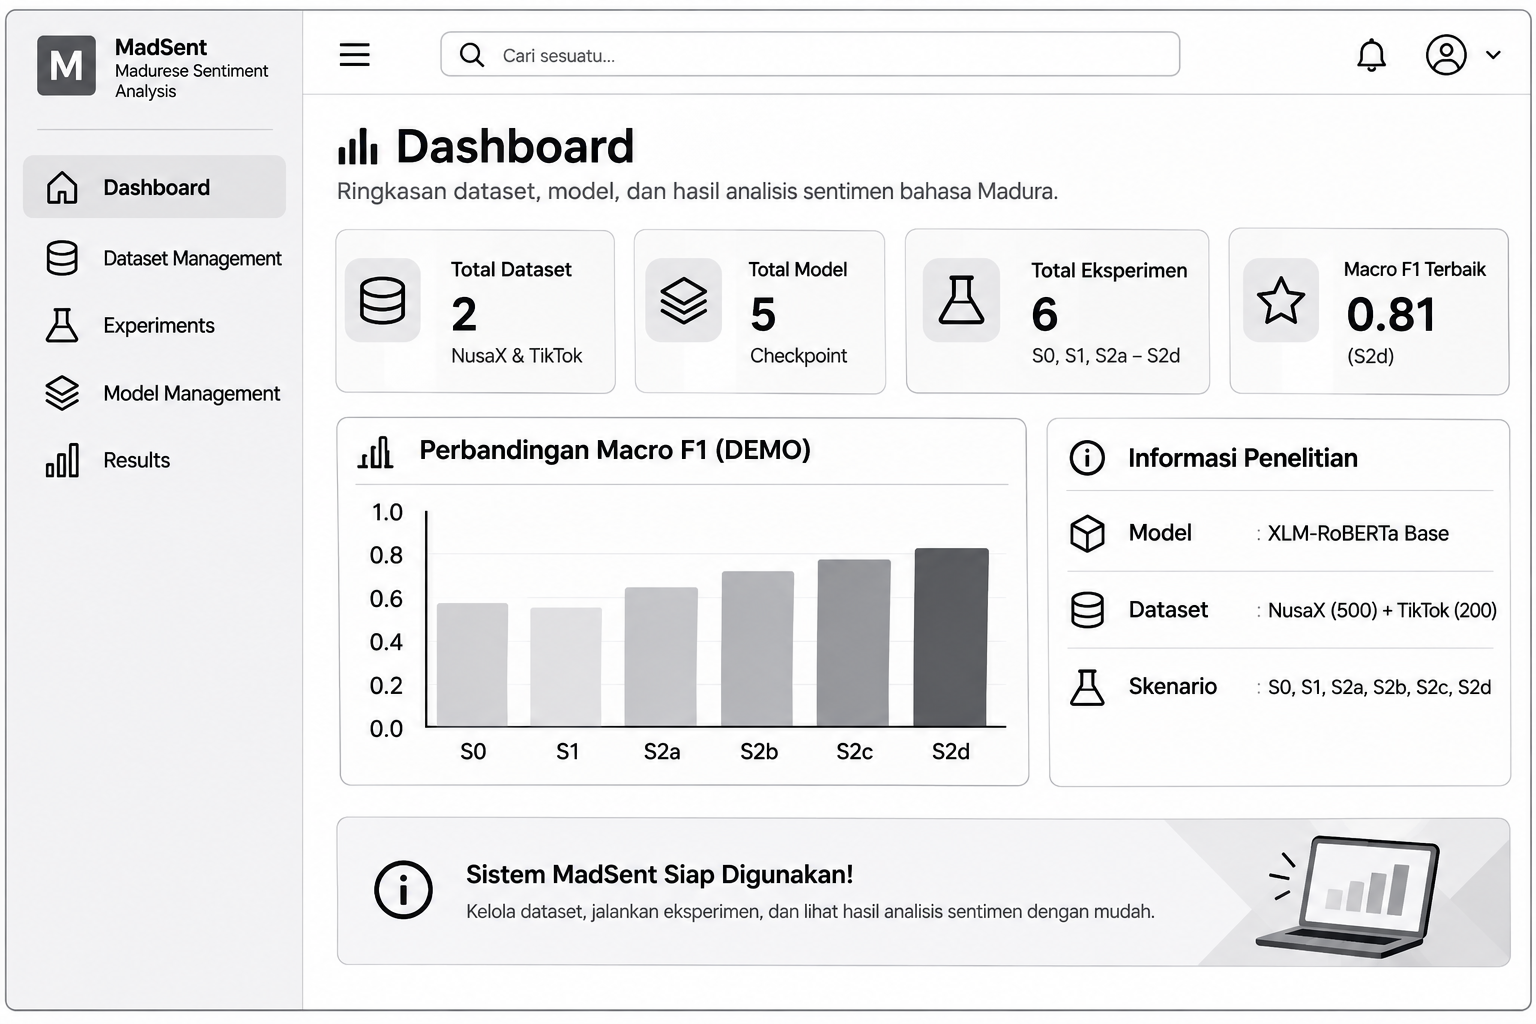
\includegraphics[width=0.68\textwidth]{figures/dashboard.png}
\caption{Rancangan Wireframe Antarmuka Modul Beranda (\textit{Dashboard})}
\label{fig:wireframe_dashboard}
\end{figure}

Sebagaimana disajikan pada \figurename~\ref{fig:wireframe_dashboard}, tata letak modul beranda memberikan gambaran komprehensif mengenai progres penelitian dan visualisasi komparatif kinerja antarskenario secara langsung, sehingga peneliti dapat memantau capaian tertinggi model secara terpadu.

\subsubsection{Modul Manajemen Data (Dataset Management)}

Modul Manajemen Data digunakan untuk mengorganisasi data teks ulasan NusaX dan komentar TikTok. Halaman ini menyediakan ringkasan volume data berlabel, fasilitas pencarian teks komentar, penyaringan berdasarkan kelas sentimen, serta tabel kurasi yang memuat ID komentar, teks bahasa Madura asli, label sentimen, dan status verifikasi. Penulis menyajikan rancangan modul manajemen data pada \figurename~\ref{fig:wireframe_dataset}.

\begin{figure}[H]
\centering
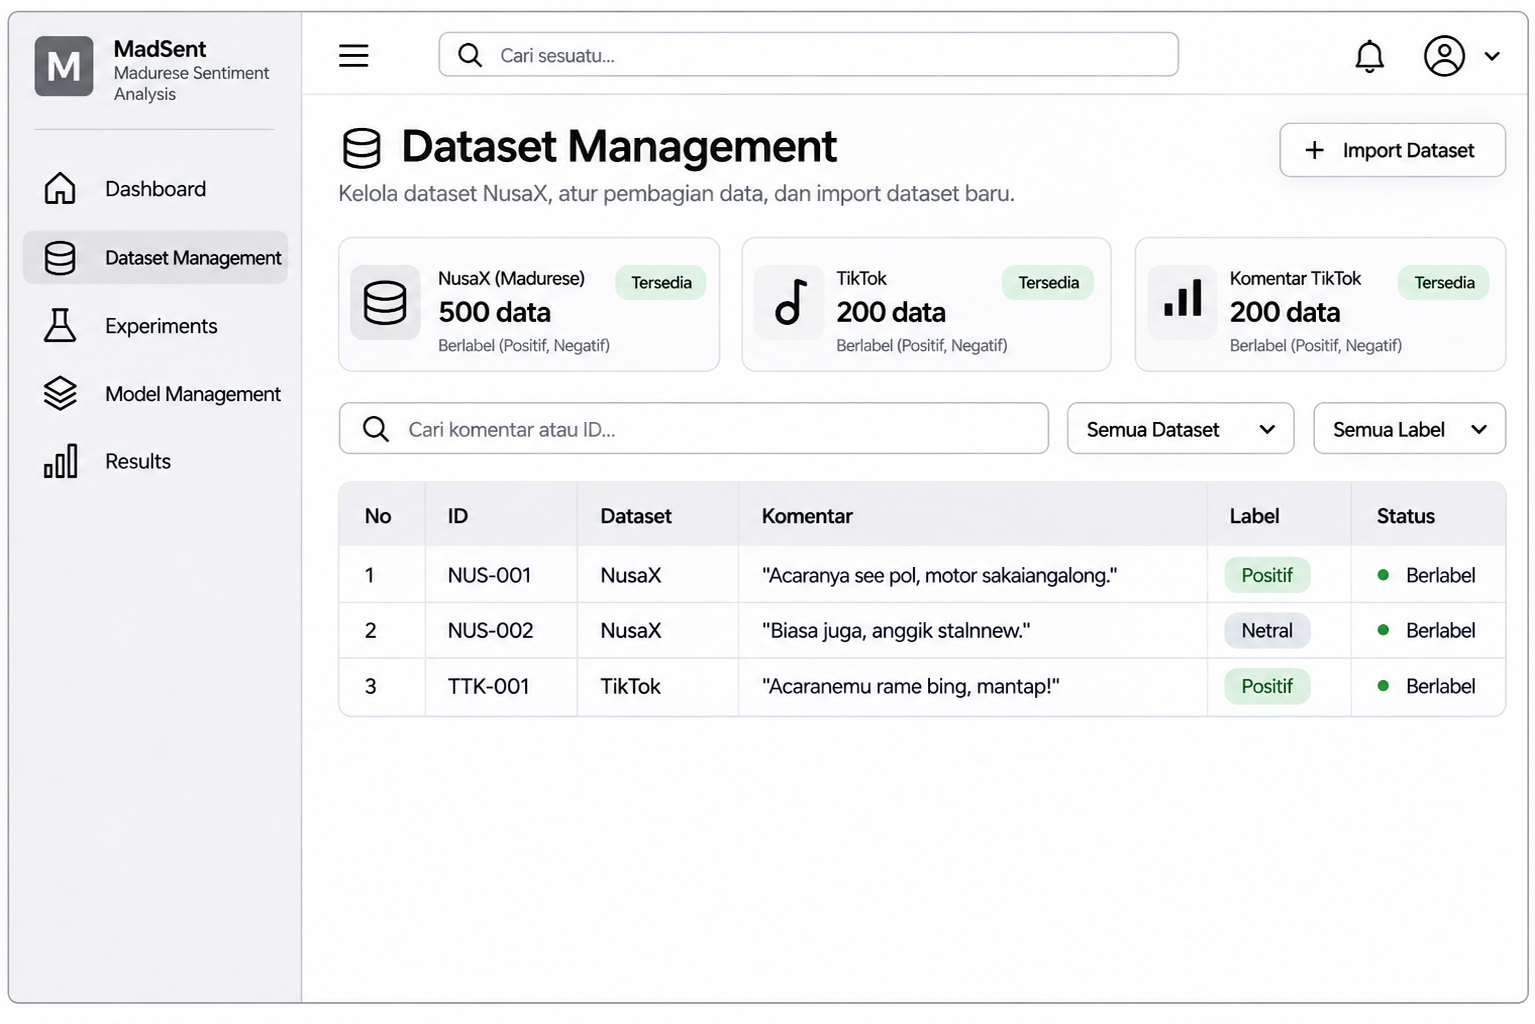
\includegraphics[width=0.68\textwidth]{figures/dataset-management.png}
\caption{Rancangan Wireframe Antarmuka Modul Manajemen Data (\textit{Dataset Management})}
\label{fig:wireframe_dataset}
\end{figure}

Sebagaimana disajikan pada \figurename~\ref{fig:wireframe_dataset}, modul manajemen data memfasilitasi penelusuran leksikon komentar daerah dan proses verifikasi label sentimen sebelum dieksekusi oleh model, serta menyediakan pemisahan tab antara korpus acuan formal dan korpus media sosial.

\subsubsection{Modul Skenario Eksperimen (Experiments)}

Modul Skenario Eksperimen mendokumentasikan keenam skenario pengujian penelitian secara runtut. Matriks eksperimen disajikan dalam format tabel interaktif yang memuat kode skenario (S0, S1, S2a, S2b, S2c, S2d), deskripsi pengujian, konfigurasi alokasi data latih, himpunan data evaluasi, dan status eksekusi. Penulis menyajikan rancangan modul skenario eksperimen pada \figurename~\ref{fig:wireframe_experiments}.

\begin{figure}[H]
\centering
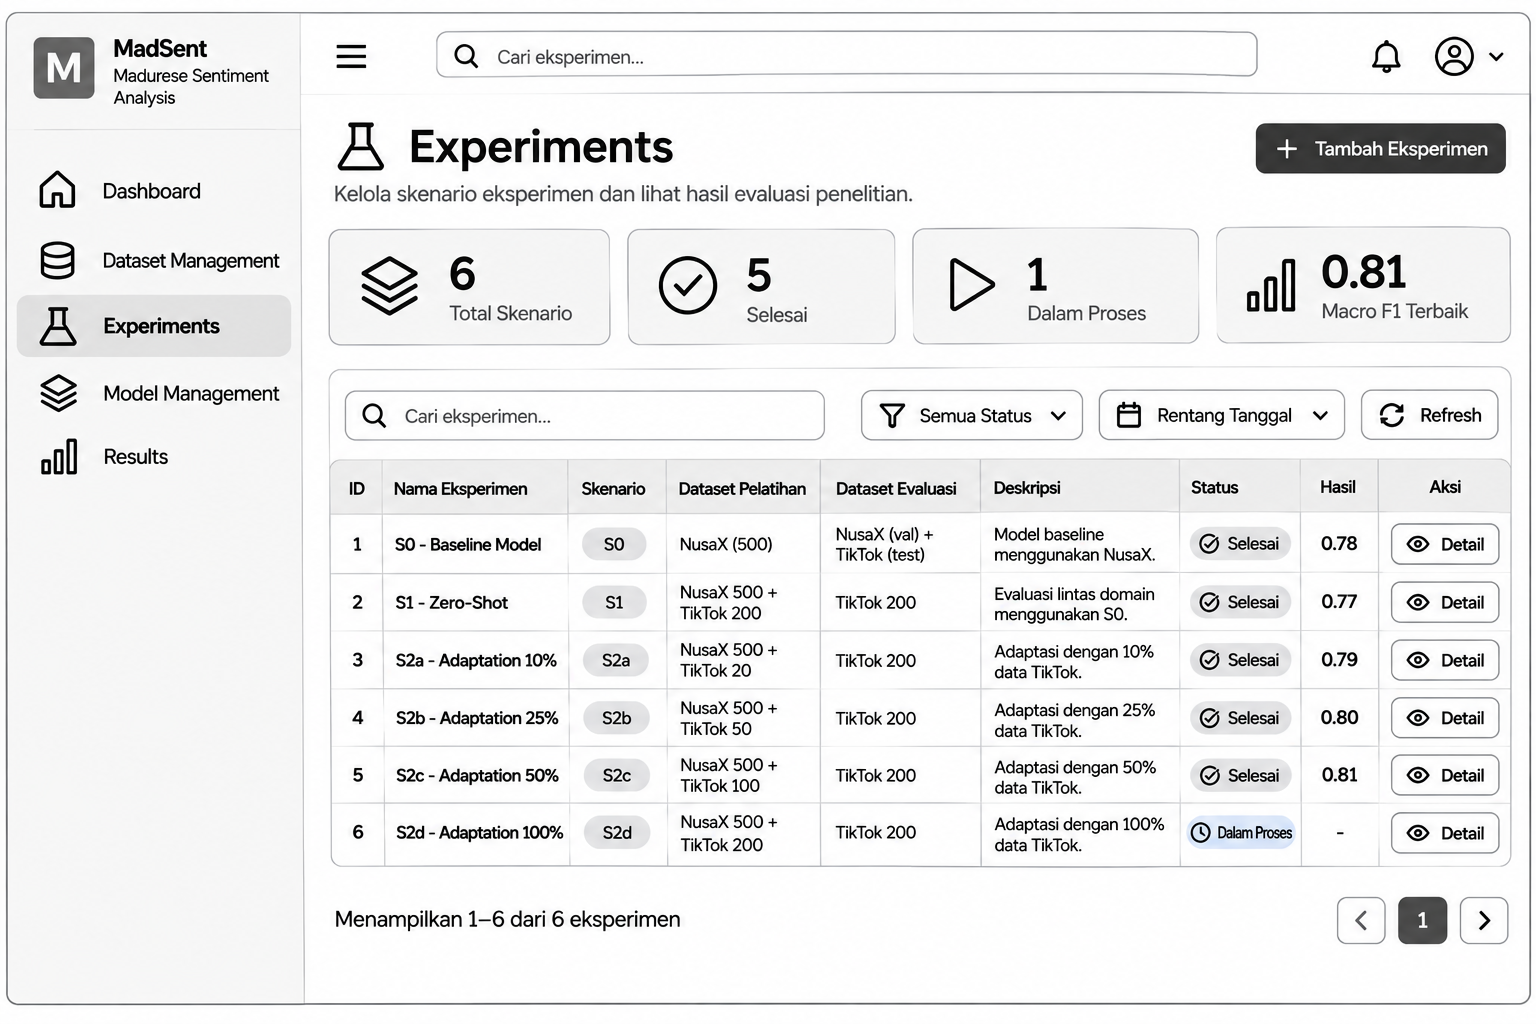
\includegraphics[width=0.68\textwidth]{figures/experiment.png}
\caption{Rancangan Wireframe Antarmuka Modul Skenario Eksperimen (\textit{Experiments})}
\label{fig:wireframe_experiments}
\end{figure}

Sebagaimana disajikan pada \figurename~\ref{fig:wireframe_experiments}, modul skenario eksperimen memastikan pencatatan konfigurasi pengujian tersimpan secara terstruktur guna mendukung replikasi hasil penelitian dan keterlacakan histori pengujian model lintas domain.

\subsubsection{Modul Manajemen Model (Model Management)}

Modul Manajemen Model berfungsi sebagai katalog pendaftaran (\textit{model registry}) untuk memantau berkas \textit{checkpoint} model XLM-RoBERTa yang telah dilatih. Pengguna dapat meninjau ketersediaan bobot model pada memori lokal, memeriksa status kesiapan pelatihan, membandingkan performa model, serta membuka laporan evaluasi model secara spesifik. Penulis menyajikan rancangan modul manajemen model pada \figurename~\ref{fig:wireframe_model}.

\begin{figure}[H]
\centering
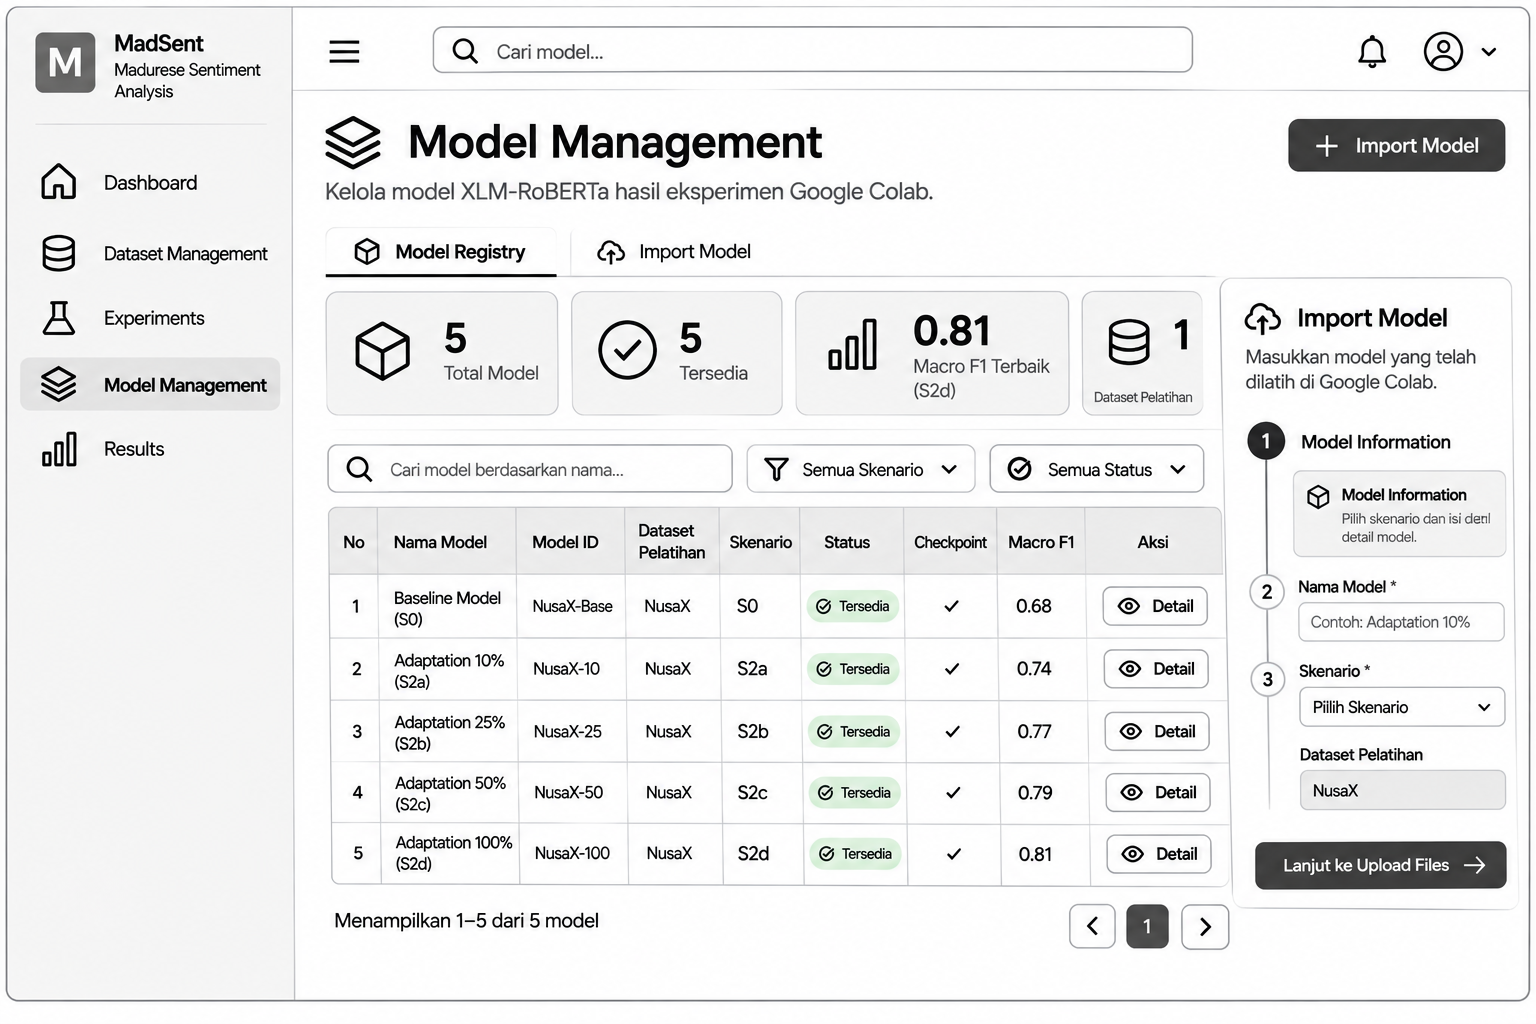
\includegraphics[width=0.68\textwidth]{figures/model-management.png}
\caption{Rancangan Wireframe Antarmuka Modul Manajemen Model (\textit{Model Management})}
\label{fig:wireframe_model}
\end{figure}

Sebagaimana disajikan pada \figurename~\ref{fig:wireframe_model}, modul manajemen model memudahkan peneliti dalam memilih dan mengaktifkan model terbaik untuk inferensi tanpa perlu melakukan pelatihan ulang, sekaligus menyediakan ringkasan metrik Macro F1 dari masing-masing checkpoint.

\subsubsection{Modul Hasil dan Evaluasi (Results)}

Modul Hasil dan Evaluasi menyajikan laporan kinerja model secara terperinci melalui kartu metrik evaluasi kuantitatif (\textit{Accuracy}, \textit{Precision}, \textit{Recall}, \textit{Macro F1-Score}), matriks konfusi interaktif tiga kelas sentimen, grafik kurva \textit{loss} pelatihan dan validasi, serta tabel analisis prediksi per komentar TikTok yang menampilkan skor keyakinan dan status kebenaran prediksi. Penulis menyajikan rancangan modul hasil dan evaluasi pada \figurename~\ref{fig:wireframe_results}.

\begin{figure}[H]
\centering
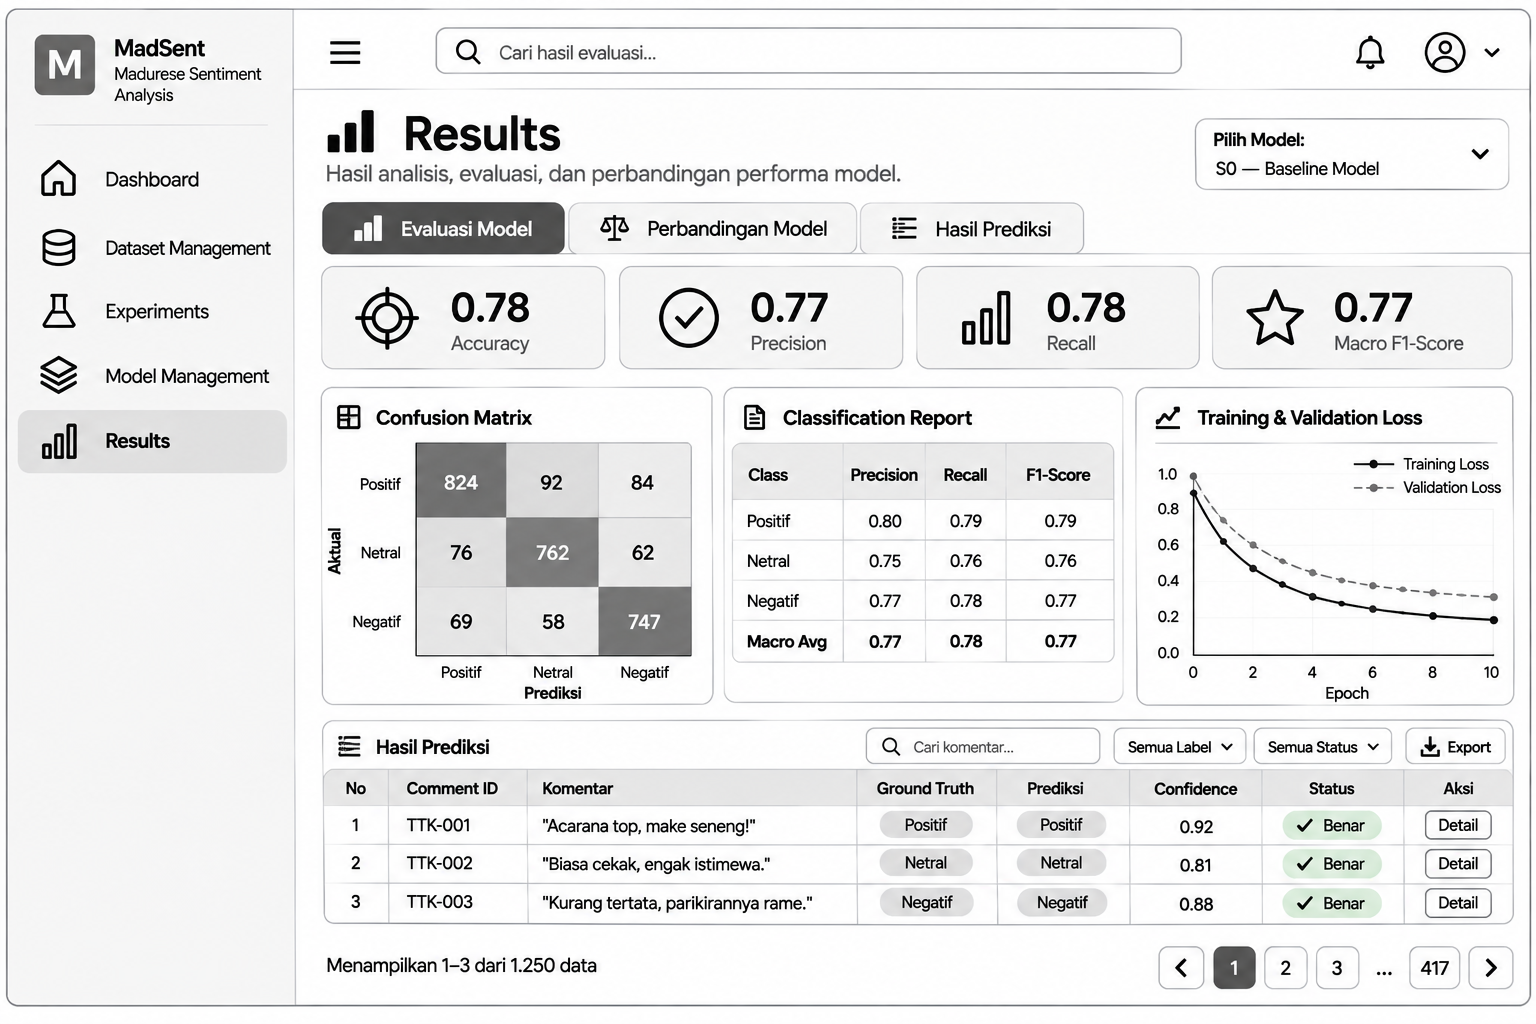
\includegraphics[width=0.68\textwidth]{figures/result.png}
\caption{Rancangan Wireframe Antarmuka Modul Hasil dan Evaluasi (\textit{Results})}
\label{fig:wireframe_results}
\end{figure}

Sebagaimana disajikan pada \figurename~\ref{fig:wireframe_results}, modul hasil dan evaluasi menyediakan sarana komprehensif bagi peneliti untuk mengidentifikasi kesalahan prediksi linguistik secara langsung pada setiap sampel komentar media sosial, sehingga memudahkan analisis mendalam pada taksonomi empat dimensi kesalahan bahasa Madura.

Melalui integrasi kelima modul antarmuka MadSent tersebut, seluruh tahapan penelitian mulai dari pengelolaan dataset, pemantauan protokol eksperimen, administrasi berkas model, hingga evaluasi kesalahan linguistik dapat dioperasikan secara terpadu dan efisien.
